\documentclass[a4paper,11pt]{article}
\usepackage{graphicx}
\usepackage[hidelinks]{hyperref}
\setcounter{tocdepth}{1}
\begin{document}
\begin{center}

\Huge\textbf{Functional Requirements\\}
																											
\vspace{2 cm}

\LARGE\textbf{Group Name:} Group 6\_b\newline
 
\vspace{0.5 cm}
\begin{tabular}{lr}
Jessica (JI) Lessev&13049136\\
Thabang (TM) Letageng&13057937\\
Michelle Swanepoel&13066294\\
Prenolan Govender&13102380\\
Fako (FJA) Peleha&12230830\\
Lutfiyya Razak&10198408\\
Ephiphania Munava&10624610\\
Maria Qumalo&29461775\\
\end{tabular}

\vspace{1cm}
\textbf{Git repository link:\\}
\url{https://github.com/u12230830/COS301\_6b}

\vspace{1cm}
\textbf{Date:} 27 February 2015
\end{center}


\newpage

\tableofcontents
\newpage
\setlength{\voffset}{-3cm}
\hspace{-1cm}The following modules will be discussed, each with their own set of use cases:
\begin{itemize}
	\item BuzzSpace Handling
	\item Thread Handling
	\item Posts Handling
	\item Filtering 
	\item Authorisation
	\item Reporting
	\item Profile Handling
\end{itemize}
\newpage
\setlength{\voffset}{-3cm}

\begin{center}
\section*\textbf\huge{BuzzSpace Handling}
\addcontentsline{toc}{section}{BuzzSpace Handling}
\\
\Large{Use Cases}
\end{center}

%-------------------------------------------------------START EDITING HERE FOR BUZZSPACE HANDLING------------------------------------------------------------
%MICHELLE
\textbf{Overview of the Domain}\\\\
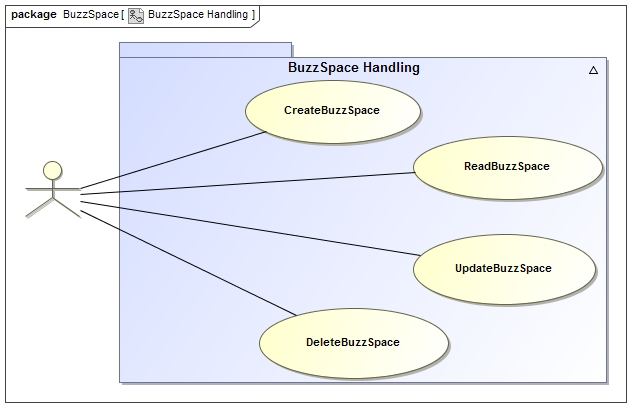
\includegraphics[width=1\linewidth]{./Images/BuzzSpaceHandling/Overview.jpg}\\
\section{Create BuzzSpace}
\subsection*{Description:}This use case encapsulates the ability for a user to create a new BuzzSpace that will be associated with a specific acitve module. 
Each BuzzSpace will have a root thread to start with. The creator of the BuzzSpace will set properties of the BuzzSpace (i.e which status is needed for a user 
to do what). 
\subsection{Prioritization:}Critical
\subsection{Conditions and Data Structures:}
\subsubsection*{Pre-Conditions:}
\begin{itemize}
	\item The user wanting to create a new BuzzSpace should be logged in to the system and should be registered with the module for which he/she wants to
	create the BuzzSpace. 
	\item The user should have a high enough status to be allowed to create a BuzzSpace (i.e. lecturer status).
	\item The module for which the BuzzSpace is being created must be an active module at that time.
\end{itemize}
\subsubsection*{Post-Conditions:}
\begin{itemize}
	\item A message is displayed to inform the creator of the BuzzSpace that the creation has been successful. Users can now start more threads on this BuzzSpace.
	\item If this service has been rejected, an exception is thrown and an error message will be displayed to the user.
\end{itemize}
\subsubsection*{Requests and Results Data Structures:}
\subsection{Required Functionality:} 
\textbf{Use case diagram of the Create BuzzSpace use case}\\ 
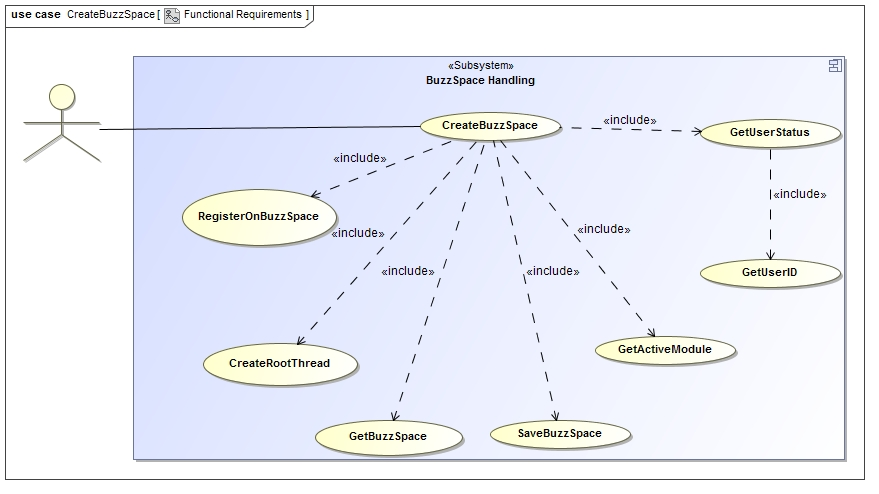
\includegraphics[width=1\linewidth]{./Images/BuzzSpaceHandling/buzzSpaceCreation.jpg}\\
\subsection{Process Specifications:} 

%MICHELLE
\section{Read BuzzSpace}
\subsection*{Description:}This use case includes the ability to view BuzzSpaces, this is, to view the different threads in the BuzzSpace (and thus have access to them), and also to view the
properties of the specific BuzzSpace (i.e. the permissions that were set, date of creation and the creator of this thread).
\subsection{Prioritization:} Critical
\subsection{Conditions and Data Structures:}
\subsubsection*{Pre-Conditions:}None 
\subsubsection*{Post-Conditions:}
\begin{itemize}
	\item Threads can now be viewed and accessed, and the properties can also be viewed.
\end{itemize}
\subsubsection*{Requests and Results Data Structures:}
\subsection{Required Functionality:} 
\textbf{Use case diagram of the Read BuzzSpace use case}\\ 
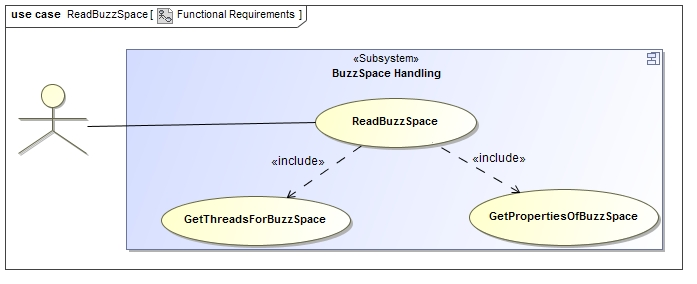
\includegraphics[width=1\linewidth]{./Images/BuzzSpaceHandling/buzzSpaceRead.jpg}\\
\subsection{Process Specifications:} 

%MICHELLE
\section{Update BuzzSpace}
\subsection*{Description:}This use case gives the ability for a user with a high enough status (lecturer status) to change the permissions needed for certain actions of this BuzzSpace. 
\subsection{Prioritization:} Important
\subsection{Conditions and Data Structures:}
\subsubsection*{Pre-Conditions:}
\begin{itemize}
	\item The user must be logged in and registered for the module that the BuzzSpace is in.
	\item The user must have lecturer status to be able to update threads.
\end{itemize}
\subsubsection*{Post-Conditions:}
\begin{itemize}
	\item A message is displayed to let the user knnow that the update has been done successfully
	\item If the service was rejected, an exception is thrown and an error message is displayed to let the user know.
\end{itemize}
\subsubsection*{Requests and Results Data Structures:}
\subsection{Required Functionality:} 
\textbf{Use case diagram of the Update BuzzSpace use case}\\
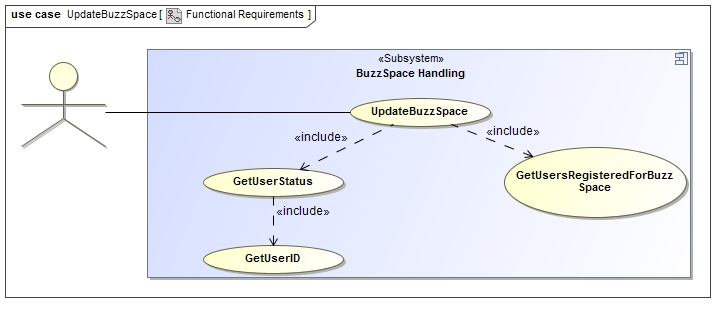
\includegraphics[width=1\linewidth]{./Images/BuzzSpaceHandling/buzzSpaceUpdate.jpg}\\
\subsection{Process Specifications:} 

%MICHELLE
\section{Delete BuzzSpace}
\subsection*{Description:}This use case includes the ability to delete a BuzzSpace when the module is not active anymore, or the BuzzSpace is not used anymore. Only the creator of the 
BuzzSpace will be able to delete a BuzzSpace, except if he changed the property to let anyone of a certain status be able to delete it.
\subsection{Prioritization:} Critical
\subsection{Conditions and Data Structures:}
\subsubsection*{Pre-Conditions:}
\begin{itemize}
	\item The user must be logged in
	\item The user must be the creator of the thread or must have a high enough status (if the permission for this was customized).
\end{itemize}
\subsubsection*{Post-Conditions:}
\begin{itemize}
	\item The BuzzSpace is deleted and archived for future reference. 
\end{itemize}
\subsubsection*{Requests and Results Data Structures:}
\subsection{Required Functionality:} 
\textbf{Use case diagram of the Delete BuzzSpace use case}\\
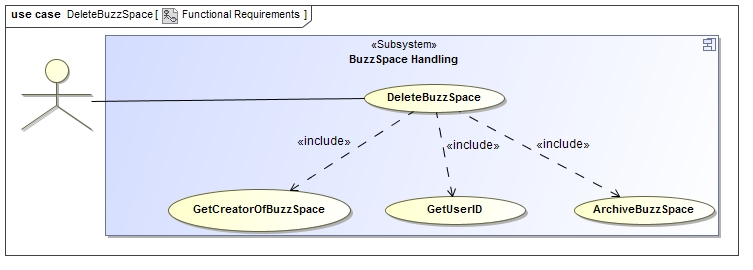
\includegraphics[width=1\linewidth]{./Images/BuzzSpaceHandling/buzzSpaceDeletion.jpg}\\
\subsection{Process Specifications:} 

%LEAVE
\newpage
\begin{center}
\section*\textbf\huge{Thread Handling}
\addcontentsline{toc}{section}{Thread Handling}
\\
\Large{Use Cases}
\end{center}
\setcounter{section}{0}

%-------------------------------------------------------START EDITING HERE FOR THREAD HANDLING------------------------------------------------------------
%JESSICA
\textbf{Overview}\\
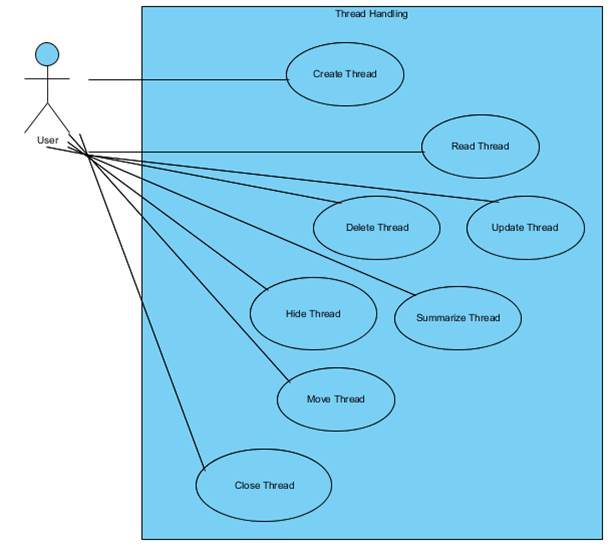
\includegraphics[width=1\linewidth]{./Images/OverviewDiagrams/ThreadHandlingOverview.jpg}\\
\section{Create Thread}
\subsection*{Description:}
1.	User activates “Create Thread” function by selecting the “Create Thread” option.\\
2.	System responds by presenting user with a form to create thread topic etc\\
3.	User fills in form ïƒ  topic of thread, tags, etc and submits the form\\
4.	System reviews the submitted information and  verifies users status and privileges, decorates the thread as needed and checks that all requirements (rules) are followed by the user based on his/her status\\
5.	 System displays either an acknowledgment or error message based on the previous checkpoint.
\subsection{Prioritization:} 
This Use case is considered Important
\subsection{Conditions and Data Structures:}
Participants:
Initiated by User and communicates with system
\subsubsection*{Pre-Conditions:}
1.	The User is logged in \\
a.	The user has a specific status
\subsubsection*{Post-Conditions:}
1.	The user fills in the form to create a new thread\\
a.	User must have a specific status in order to perform certain functions when creating a thread
\subsubsection*{Requests and Results Data Structures:}
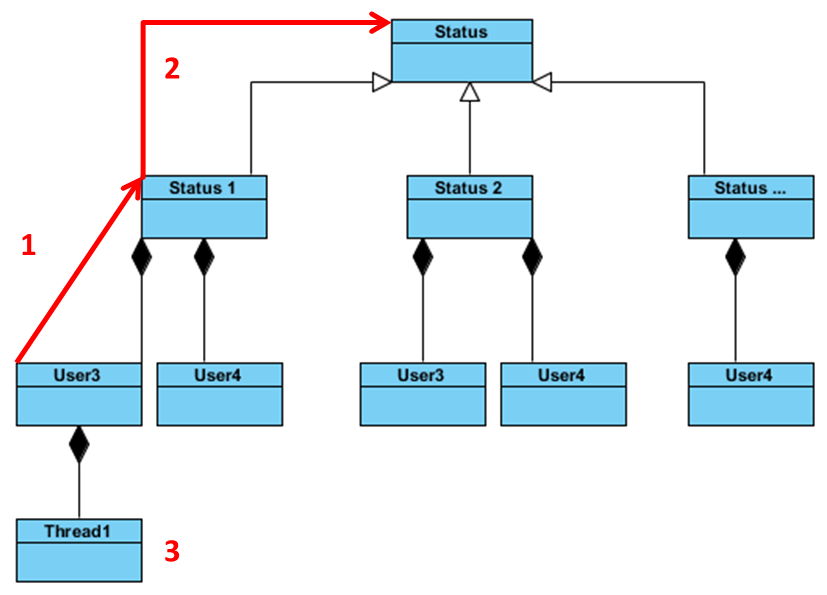
\includegraphics[width=\linewidth]{./Images/CRUDThread/Diagrams/1.png}
Status can be an abstract class and each sub-class will be a generalization of this class as each new status “IS-A” status.
Each user “HAS-A” status and thus each new user will be a composition of each specific status class.
Each thread “HAS-A” user that started it and thus each new thread will be a composition of each user.\\
Steps:\\
1.	If the user attempts to create a thread, the system will first check if the user is logged in.\\
1.1.	If so, it will go to number 1 above and check the users status\\
1.1.1.	The system verifies the status and at number 2 checks that the user has the privileges to create threads of the appropriate size, contents etc.\\
1.1.1.1	If the user has the necessary privileges then the thread is created at 3\\
1.1.1.2	Otherwise an error message is displayed telling the user that he/she does not have the necessary privileges \\
2.	If the user is not logged in, an error message is displayed telling the user that he/she is not logged in and it will redirect to the logging page.\\
\subsection{Required Functionality:} 
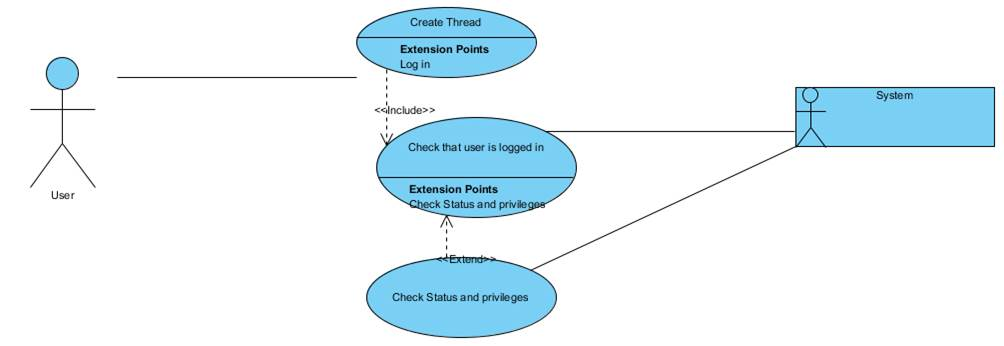
\includegraphics[width=\linewidth]{./Images/CRUDThread/Diagrams/2.jpg}
\subsection{Process Specifications:} 
Activity Diagram\\
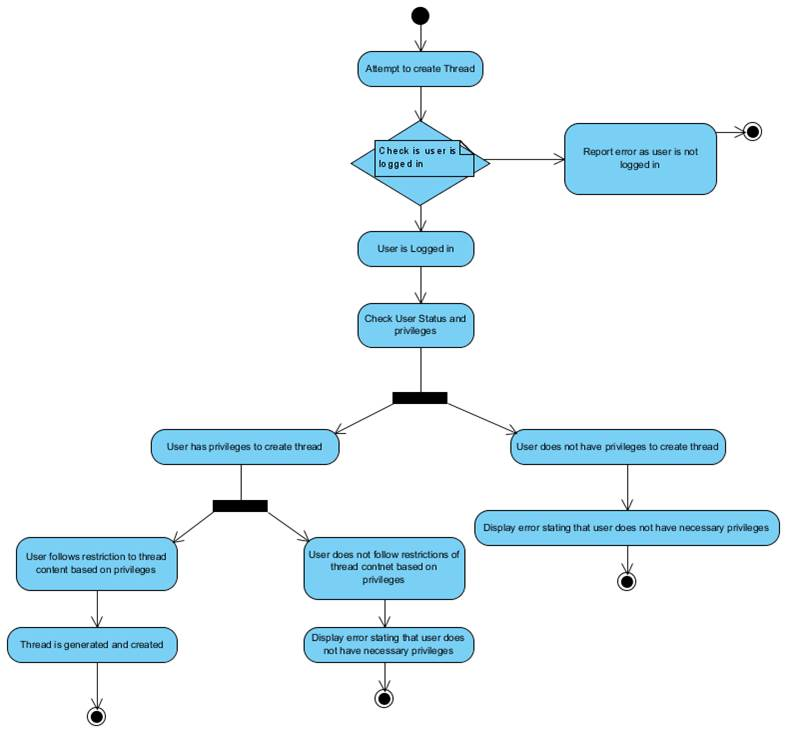
\includegraphics[width=\linewidth]{./Images/CRUDThread/Diagrams/3.jpg}
\newpage
Sequence Diagram\\
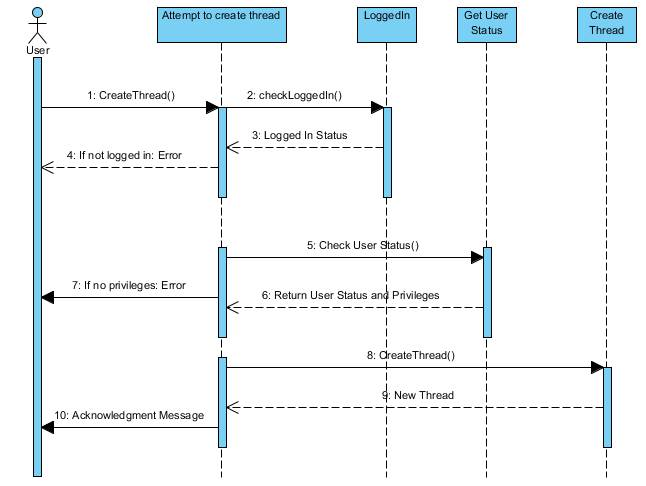
\includegraphics[width=1\linewidth]{./Images/CRUDThread/Diagrams/4.jpg}\\

%JESSICA
\section{Read Thread}
\subsection*{Description:}
1.	User activates “Read Thread” function by selecting the “A Thread” they wish to read.\\
2.	System responds by presenting user with the selected thread of posts\\
3.	User reads the posts and based on privileges can make changes such as update, delete, reply, tag, rate etc\\

\subsection{Prioritization:}
This Use case is considered Important\\ 
\subsection{Conditions and Data Structures:}
Participants:\\
Initiated by User and communicates with system\\
\subsubsection*{Pre-Conditions:}
1.	The user must click on a thread they wish to read\\
1.1.	If User is logged in and\\
1.1.1.	User has status with high privileges then the user has options to change thread\\
1.1.1.1.	Calls other use cases\\
1.1.2.	Otherwise user is automatically logged in as “Guest” and can only view posts
\subsubsection*{Post-Conditions:}
1.	System displays selected thread with posts\\
2.	If user is logged on and has privileges then an attempt to make changes such as update, delete, reply, tag, rate etc will be acknowledged. 

\subsubsection*{Requests and Results Data Structures:}
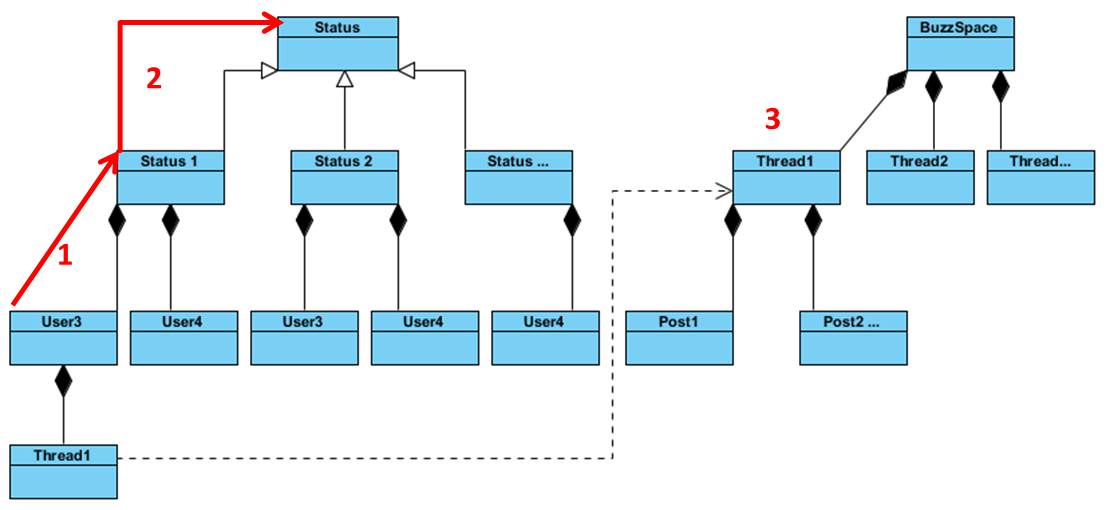
\includegraphics[width=1\linewidth]{./Images/CRUDThread/Diagrams/5.jpg}\\
Status can be an abstract class and each sub-class will be a generalization of this class as each new status “IS-A” status.\\
Each user “HAS-A” status and thus each new user will be a composition of each specific status class.\\
Each thread “HAS-A” user that started it and thus each new thread will be a composition of each user.\\
Each thread “HAS-A” BuzzSpace and thus each new thread will be a composition of each BuzzSpace.\\
Each Post “HAS-A” Thread and thus each new post will be a composition of each Thread\\\\

Steps:\\
1.	If the user attempts to enter a thread to read then the system will first check if the user is logged in.\\
1.1.	If so it will go to number 3 and open the selected thread to read.\\
1.1.1.	If user attempts to alter a post it will go to number 1 above and check the users status\\
1.1.1.1.	The system verifies the status and at number 2 checks that the user has the privileges to create threads of the appropriate size, contents etc.\\
1.1.1.2.	If the user has the necessary privileges then the post is altered at 3\\
1.1.1.3.	Otherwise an error message is displayed telling the user that he/she does not have the necessary privileges \\
1.2.	If not the user will be automatically logged on as “Guest”


\subsection{Required Functionality:} 
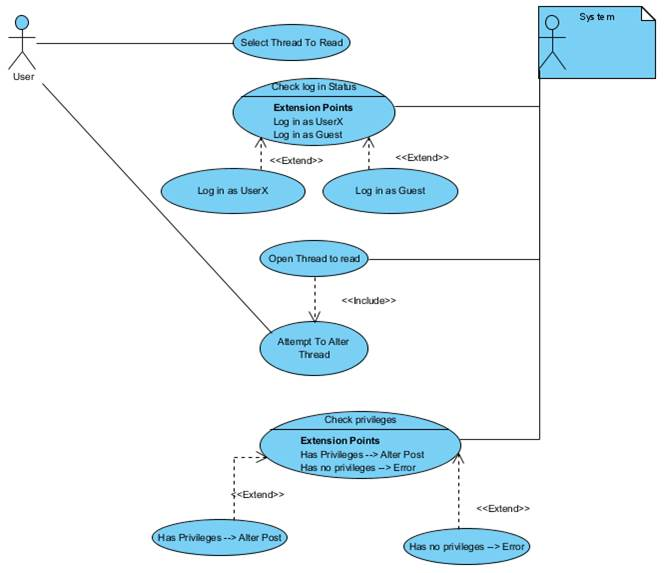
\includegraphics[width=1\linewidth]{./Images/CRUDThread/Diagrams/6.jpg}\\
\subsection{Process Specifications:} 
Activity Diagram\\
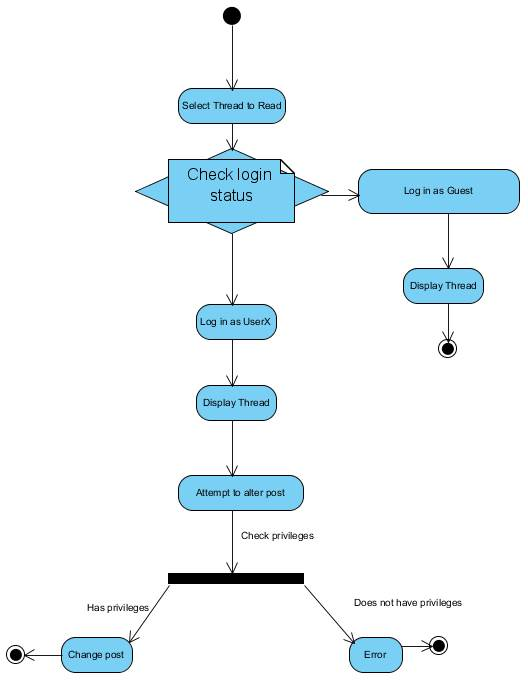
\includegraphics[width=1\linewidth]{./Images/CRUDThread/Diagrams/7.jpg}\\
\newpage
Sequence Diagram\\
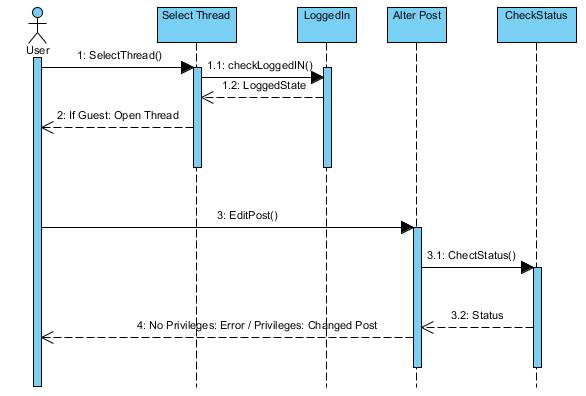
\includegraphics[width=1\linewidth]{./Images/CRUDThread/Diagrams/8.jpg}\\

%JESSICA
\section{Update Thread}
\subsection*{Description:}
1.	User activates “Update Thread” function by selecting the “Update Thread” option by choosing how they wish to update the thread.\\
2.	System checks to see whether user is logged in\\
3.	System reviews the submitted information and  verifies users status and privileges, decorates the thread as needed and checks that all requirements (rules) are followed by the user based on his/her status\\
4.	 System displays either an acknowledgment or error message based on the previous checkpoint.\\

\subsection{Prioritization:} 
This Use case is considered Important\\
\subsection{Conditions and Data Structures:}
Participants:\\
Initiated by User and communicates with system\\
\subsubsection*{Pre-Conditions:}
1.	User chooses the way in which to update a thread\\
2.	The User is logged in \\
2.1.	The user has a specific status\\
2.2.	User must have a specific status in order to perform certain functions when updating a thread\\
\subsubsection*{Post-Conditions:}
1.	System displays an acknowledgment message and updates  the new thread  if user follows “status based rules”\\
2.	Systems display an error message and requests user to restart if user attempts to perform a function that is not within the scope of their status privileges.\\
\subsubsection*{Requests and Results Data Structures:}
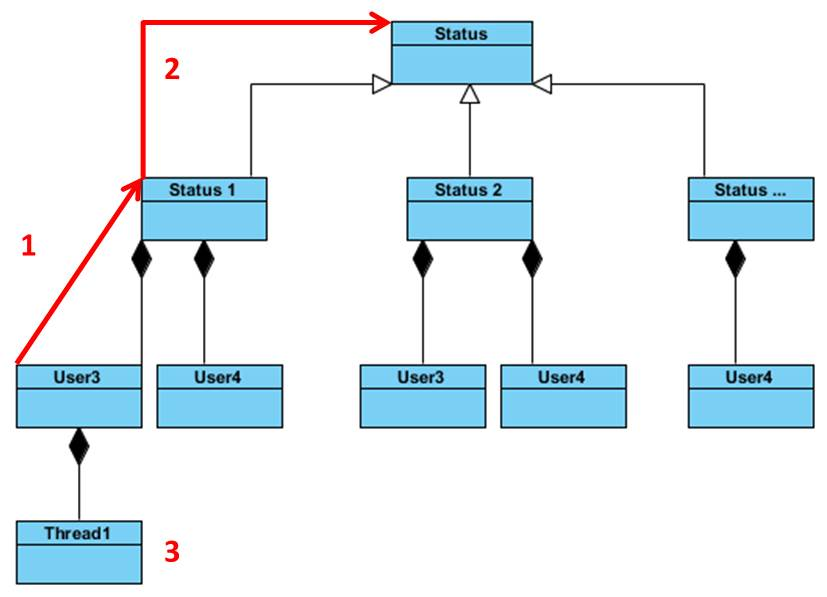
\includegraphics[width=1\linewidth]{./Images/CRUDThread/Diagrams/9.jpg}\\
Status can be an abstract class and each sub-class will be a generalization of this class as each new status “IS-A” status.\\
Each user “HAS-A” status and thus each new user will be a composition of each specific status class.\\
Each thread “HAS-A” user that started it and thus each new thread will be a composition of each user.\\
Steps:\\
1.	If the user attempts to update a thread, the system will first check if the user is logged in.\\
1.1.	If so, it will go to number 1 above and check the users status\\
1.1.1.	The system verifies the status and at number 2 checks that the user has the privileges to update threads in the specific way chosen.\\
1.1.1.1.	If the user has the necessary privileges then the thread is updated at 3\\
1.1.1.2.	Otherwise an error message is displayed telling the user that he/she does not have the necessary privileges \\
1.2.	If the user is not logged in, an error message is displayed telling the user that he/she is not logged in and it will redirect to the logging page.\\
\subsection{Required Functionality:}
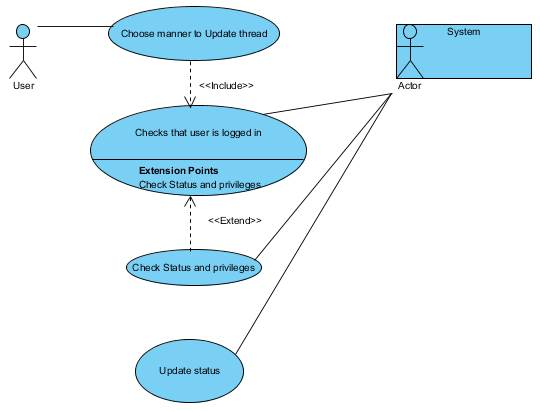
\includegraphics[width=1\linewidth]{./Images/CRUDThread/Diagrams/10.jpg}\\
\subsection{Process Specifications:} 
Activity Diagram\\
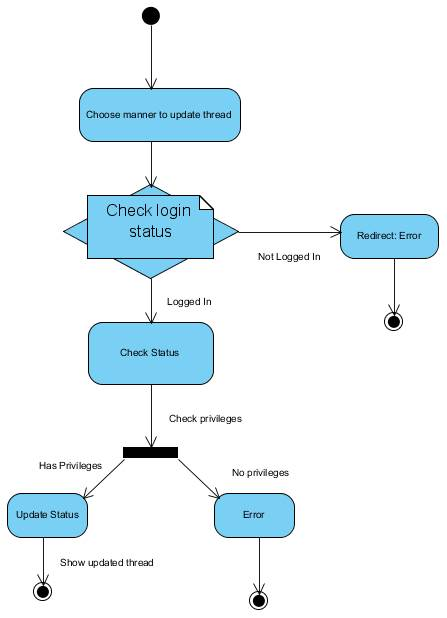
\includegraphics[width=1\linewidth]{./Images/CRUDThread/Diagrams/11.jpg}\\
\newpage
Sequence Diagram\\
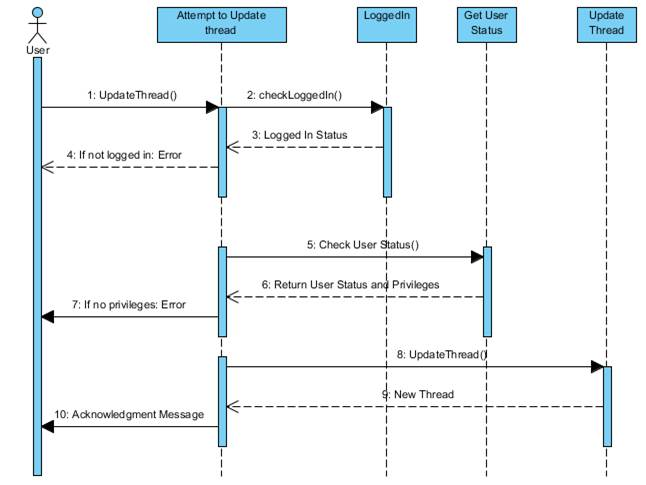
\includegraphics[width=1\linewidth]{./Images/CRUDThread/Diagrams/12.jpg}\\

%JESSICA
\section{Delete Thread}
\subsection*{Description:}
1	User activates “Delete Thread” function by selecting the “Delete Thread” option.\\
2	System checks to see whether user is logged in\\
3	System reviews the submitted information and  verifies users status and privileges\\
4	System displays either an acknowledgement and removes the thread or displays an error message based on the pervious checkpoint.\\
\subsection{Prioritization:} 
This Use case is considered Important\\
\subsection{Conditions and Data Structures:}
Participants:\\
Initiated by User and communicates with system\\
\subsubsection*{Pre-Conditions:}
1.	User selects “Delete Thread” \\
2.	The User is logged in \\
2.1.	The user has a specific status\\
2.2.	User must have a specific status in order to delete a thread\\
\subsubsection*{Post-Conditions:}
1.	System displays an acknowledgment message and removes  the thread  if user follows “status based rules”\\
2.	Systems display an error message and requests user to restart if user attempts to perform a function that is not within the scope of their status privileges.\\
\subsubsection*{Requests and Results Data Structures:}
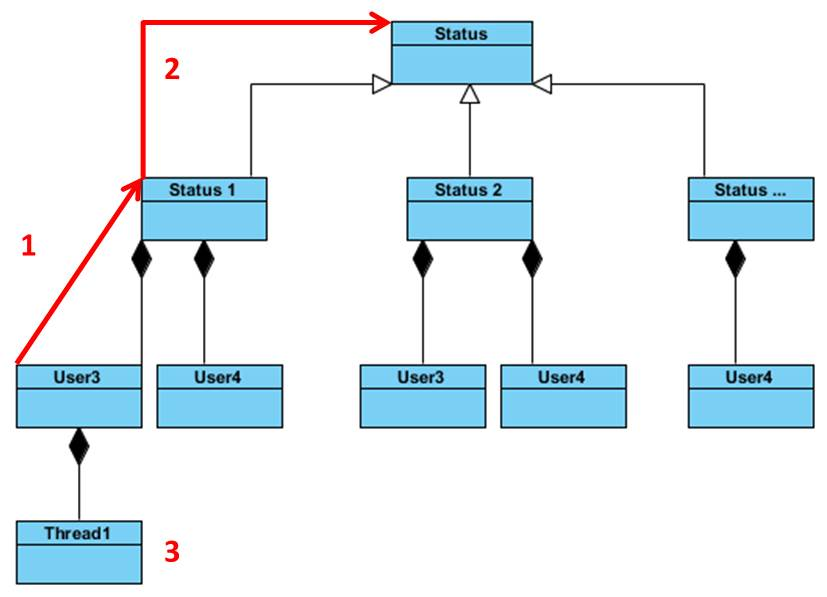
\includegraphics[width=1\linewidth]{./Images/CRUDThread/Diagrams/13.jpg}\\
Status can be an abstract class and each sub-class will be a generalization of this class as each new status “IS-A” status.\\
Each user “HAS-A” status and thus each new user will be a composition of each specific status class.\\
Each thread “HAS-A” user that started it and thus each new thread will be a composition of each user.\\
Steps:\\
1.	If the user attempts to delete a thread, the system will first check if the user is logged in.\\
1.1.	If so, it will go to number 1 above and check the users status\\
1.1.1.	The system verifies the status and at number 2 checks that the user has the privileges to delete thread.\\
1.1.1.1.	If the user has the necessary privileges then the thread at 3 is removed from the tree\\
1.1.1.2.	Otherwise an error message is displayed telling the user that he/she does not have the necessary privileges \\
1.2.	If the user is not logged in, an error message is displayed telling the user that he/she is not logged in and it will redirect to the logging page.\\
\subsection{Required Functionality:} 
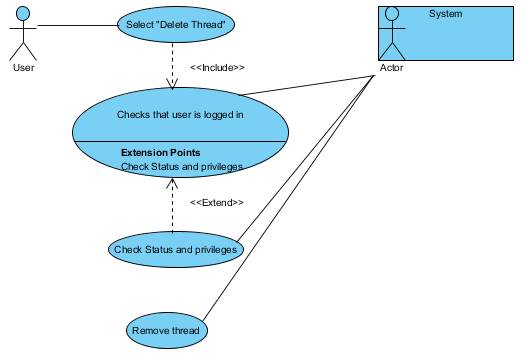
\includegraphics[width=1\linewidth]{./Images/CRUDThread/Diagrams/14.jpg}\\
\subsection{Process Specifications:} 
Activity Diagram\\
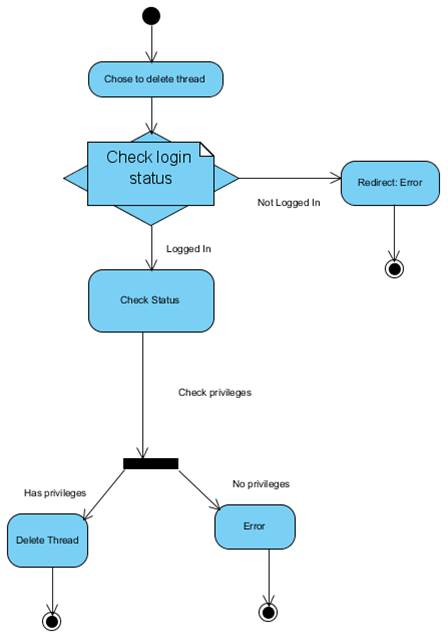
\includegraphics[width=1\linewidth]{./Images/CRUDThread/Diagrams/15.jpg}\\
\newpage
Sequence Diagram\\
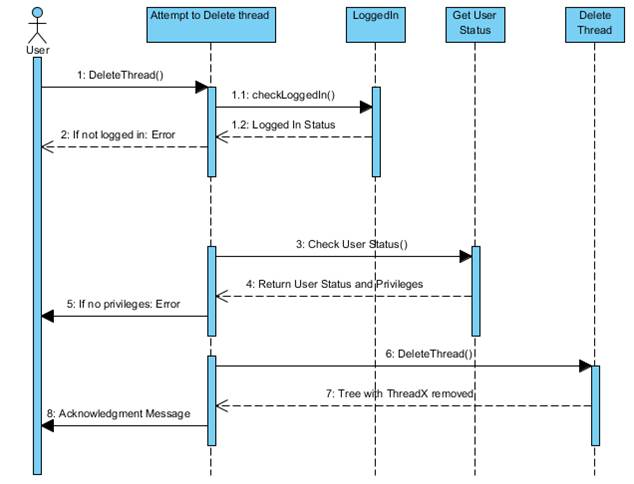
\includegraphics[width=1\linewidth]{./Images/CRUDThread/Diagrams/16.jpg}\\


%JIMMY
\section{Summarise Thread}
\subsection*{Description:}
Since a thread can, in theory, grow infinitely long, It is therefor necessary to show only the important aspects of the thread. These are the root post in the thread, the declared answer in the thread and the thread's social tags.\\
\subsection{Prioritization:}
This feature is Nice-To-Have. The system will not be immensely devalued if this feature is not added.\\ 
\subsection{Conditions and Data Structures:}
\subsubsection*{Pre-Conditions:}
1.	The thread must be closed (No longer open for discussion).\\
2.	User must be logged on as the system administrator to summarise a thread.\\
3.	The thread must be more than 3 posts long.\\
\subsubsection*{Post-Conditions:}
1.	The thread is summarised successfully if all pre-conditions are me.\\
2.	The system displays an error message if at least one of the pre-conditions are violated.\\
\subsubsection*{Requests and Results Data Structures:}
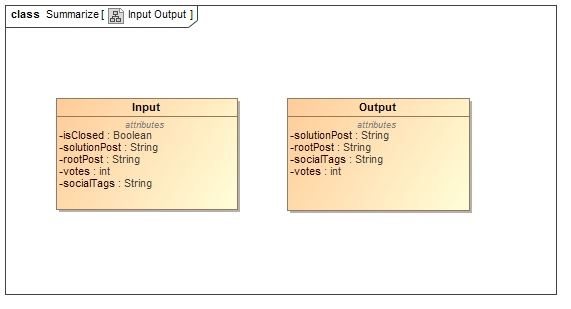
\includegraphics{Images/SCHMThread/SummarizeInOut.jpg}\\
\subsection{Required Functionality:} 
Summarizing a thread\\
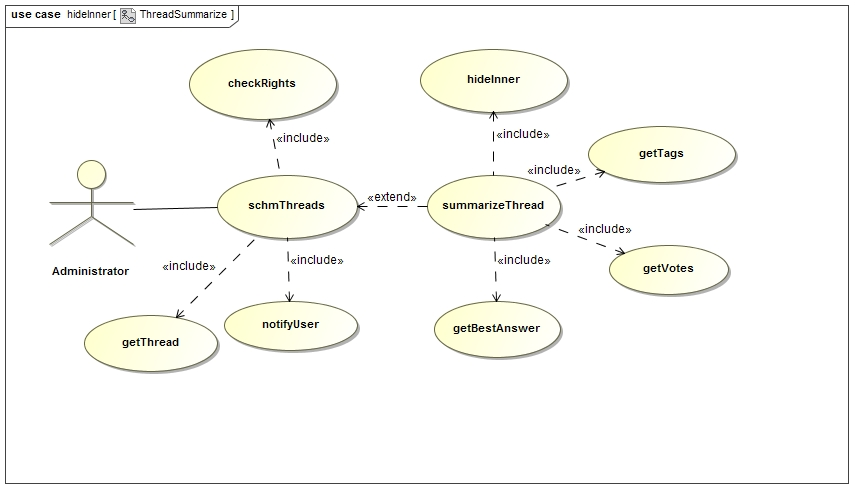
\includegraphics[width=1\linewidth]{./Images/SCHMThread/ThreadSummarize.jpg}\\
\subsection{Process Specifications:} 
%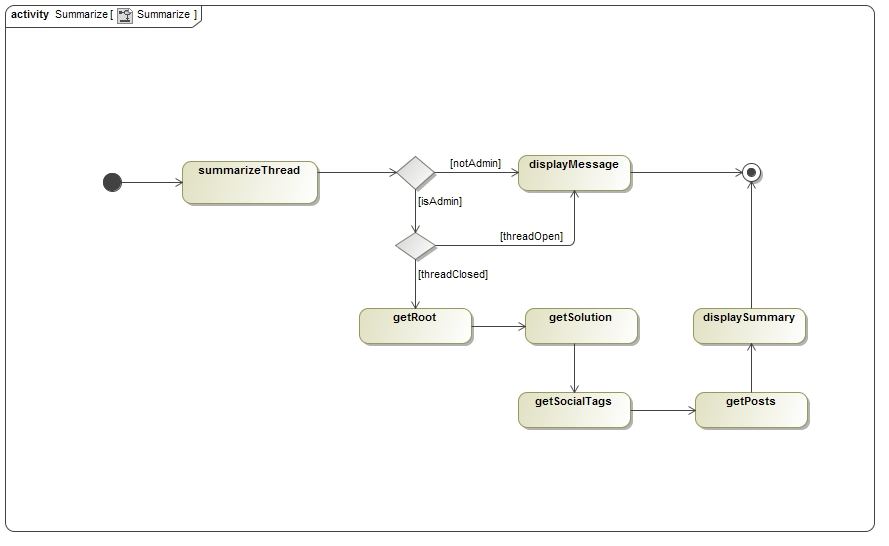
\includegraphics[width=1.2\linewidth]{./Images/BestAnswer/SummarizeAct.jpg}\\

%JIMMY
\section{Hide Thread}
\subsection*{Description:}
Hiding a thread is when the System administrator makes the thread invisible to the user but not to the system. It is necessary for cases like when a thread is under plagiarism investigations or when the discussion is considered inappropriate. It will still exist in the Buzz space but users will not see it and, in turn, add onto it. \\
\subsection{Prioritization:}
It is considered critical to the system. It remains key that the system maintains its credibility and integrity at all times. This avoids conflicts and legal issues that may arise.\\ 
\subsection{Conditions and Data Structures:}
\subsubsection*{Pre-Conditions:}
1.	The user must be logged on as a system administrator.\\
2.	The thread must have been flagged by the system for plagiarism or other questionable characteristics such as vulgar language or slander.\\
\subsubsection*{Post-Conditions:}
1.	The thread is successfully hidden from the user if all pre-conditions are met.\\
2.	The thread is still visible to the system.\\
3.	A notification is sent to the owner of the thread that it is pending investigation.\\
4.	The thread remains unhidden and an error message is shown if at least one of the pre-conditions aren't met.\\
\subsubsection*{Requests and Results Data Structures:}
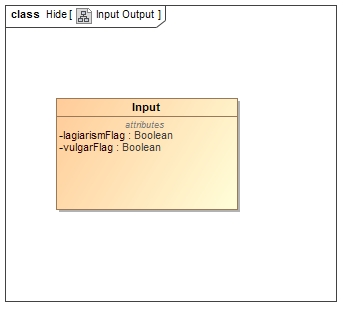
\includegraphics{Images/SCHMThread/HideInOut.jpg}\\
\subsection{Required Functionality:} 
Hiding a thread.\\
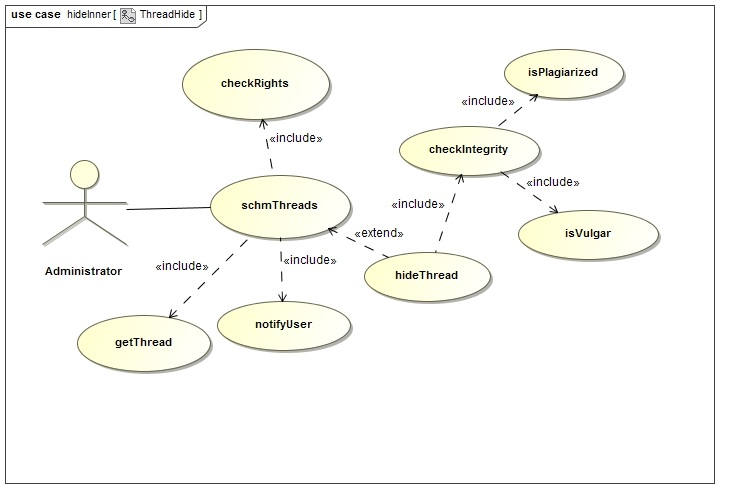
\includegraphics[width=1\linewidth]{./Images/SCHMThread/ThreadHide.jpg}\\
\subsection{Process Specifications:} 
%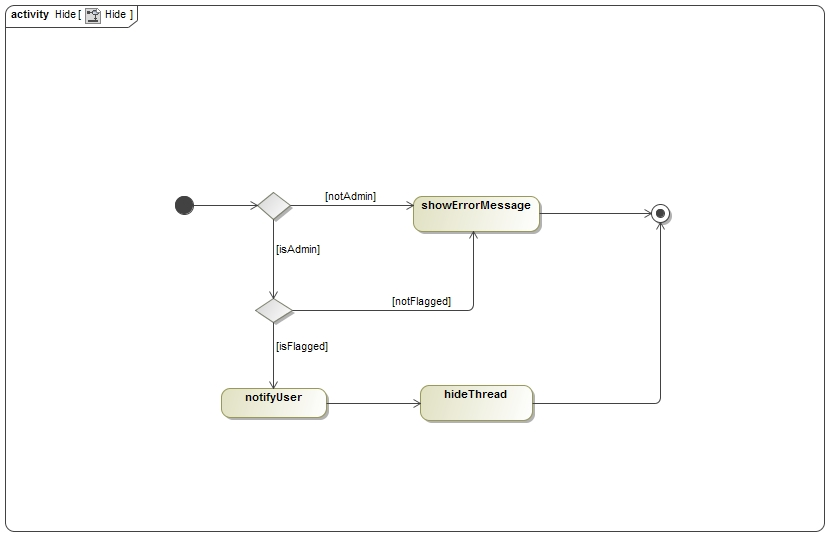
\includegraphics[width=1.2\linewidth]{./Images/BestAnswer/HideAct.jpg}\\

%JIMMY
\section{Close Thread}
\subsection*{Description:}
Once a best answer has been agreed upon by the thread owner and users, it is no longer necessary for the thread to be open to discussion. It is therefore preferable for it to be available for viewing and not commenting on. It is considered closed when this happens. \\
\subsection{Prioritization:}
This feature is considered important. The system can cope without it but it is not preferable because threads can grow to be very long.\\
\subsection{Conditions and Data Structures:}
\subsubsection*{Pre-Conditions:}
1.	The user must be logged in as an administrator.\\
2.	The a best answer has to have been chosen by the thread owner based on his or her discretion and votes from the users.\\
\subsubsection*{Post-Conditions:}
1.	An error message is shown if at least one of the pre-conditions have been violated.\\
2.	The thread is closed successfully if the pre-conditions have been met or open otherwise.\\
3.	User is notified that thread is closed.\\
\subsubsection*{Requests and Results Data Structures:}
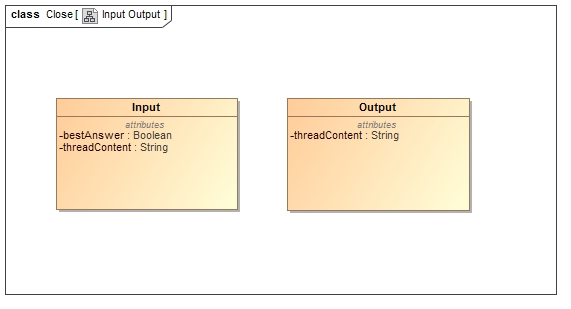
\includegraphics{Images/SCHMThread/CloseInOut.jpg}\\
\subsection{Required Functionality:} 
Closing a thread.\\
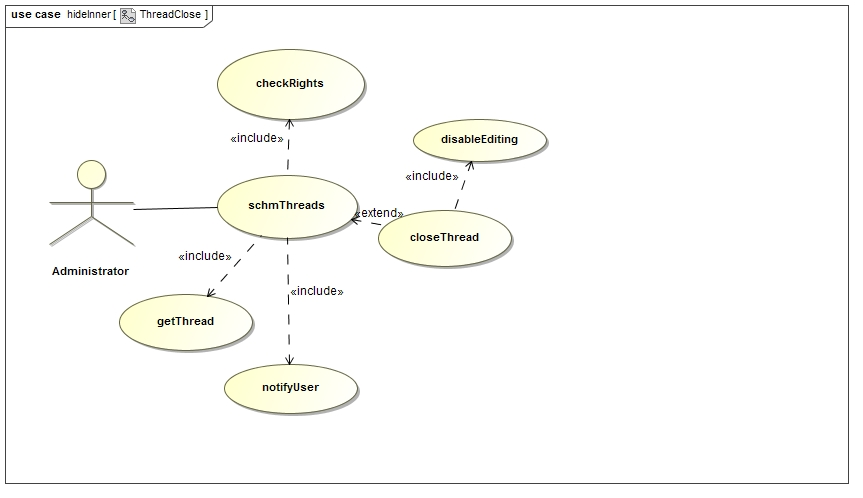
\includegraphics[width=1\linewidth]{./Images/SCHMThread/ThreadClose.jpg}\\
\subsection{Process Specifications:}
%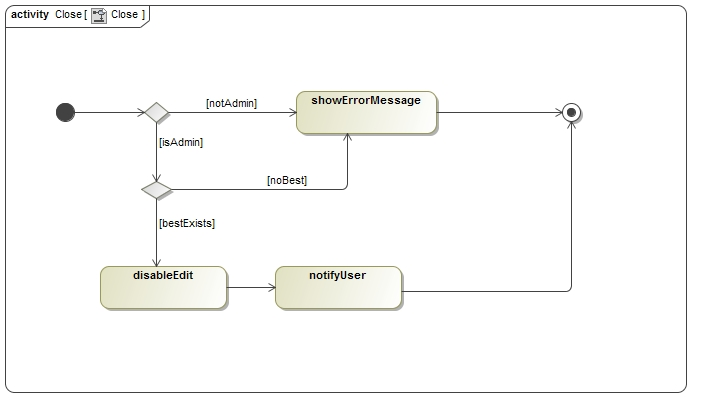
\includegraphics[width=1.2\linewidth]{./Images/BestAnswer/CloseAct.jpg}\\

%JIMMY
\section{Move Thread}
\subsection*{Description:}
Moving a thread can entail either deleting it from its original Buzz space to a different one or duplicating it. The former is necessary when a thread is not relevant to the Buzz space in question while the latter is important when it is relevant to both.\\
\subsection{Prioritization:} 
\subsection{Conditions and Data Structures:}
\subsubsection*{Pre-Conditions:}
1.	The user must be logged in as an administrator.\\
2.	The thread owner must have given consent for the contents of the thread to be moved.\\
\subsubsection*{Post-Conditions:}
1.	An error message is displayed if the user is not logged on as admin.\\
2.	The thread is successfully moved if both pre-conditions are met.\\
3.	The thread owner is notified if the thread is successfully moved.\\
\subsubsection*{Requests and Results Data Structures:}
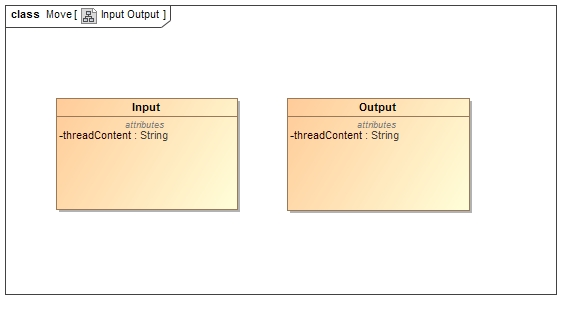
\includegraphics{Images/SCHMThread/MoveInOut.jpg}\\
\subsection{Required Functionality:} 
Moving a thread.\\
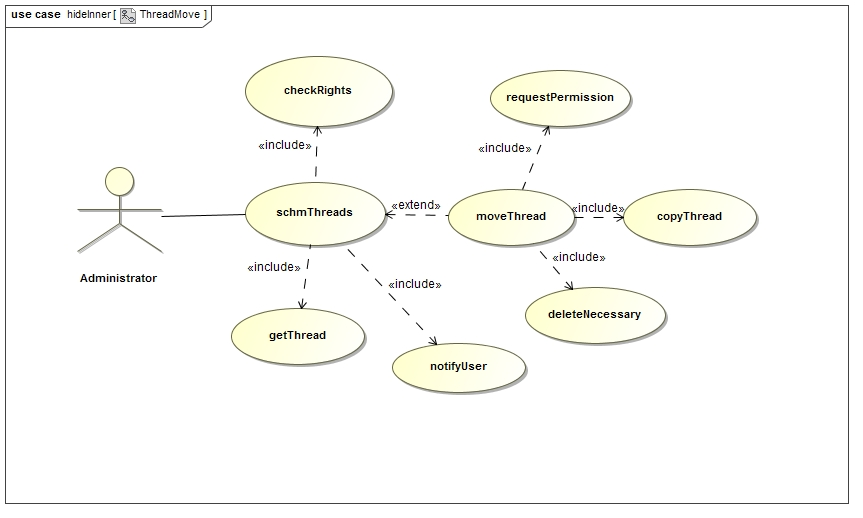
\includegraphics[width=1\linewidth]{./Images/SCHMThread/ThreadMove.jpg}\\
\subsection{Process Specifications:} 
%\includegraphics[width=1.2\linewidth]{./Images/BestAnswer/MoveAct.jpg}\\

%LEAVE
\newpage
\begin{center}
\section*\textbf\huge{Post Handling}
\addcontentsline{toc}{section}{Post Handling}
\\
\Large{Use Cases}
\end{center}
\setcounter{section}{0}
%---------------------------------------------------------------START EDITING HERE FOR POST HANDLING----------------------------------------------------------------------
%MICHELLE
\textbf{Overview of the Domain}\\\\
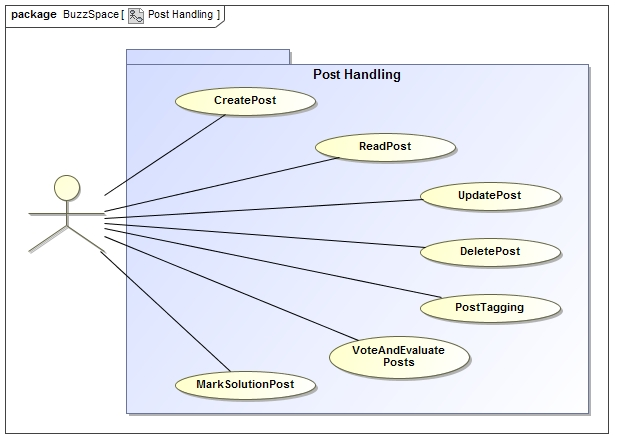
\includegraphics[width=1\linewidth]{./Images/PostHandling/Overview.jpg}\\
\section{Create Post}
\subsection*{Description:}This use case refers to the ability to create a new post on a certain thread. 
\subsection{Prioritization:} Critical
\subsection{Conditions and Data Structures:}
\subsubsection*{Pre-Conditions:}
\begin{itemize}
	\item The user must be logged in and registered to the specific BuzzSpace in which the post is created
	\item The user must adhere to the specifications of which user status levels can create a post on which level at which length.
\end{itemize}
\subsubsection*{Post-Conditions:}
\begin{itemize}
	\item If the user did not adhere to the specifications of which user status levels can create a post on which level at which length, an exception will be thrown and an error
	message will be displayed to the user.
	\item if plagiarism was detected on the post, then the service is rejected and an exception is thrown with an error message is displayed to the user.
	\item If netiquette rules were broken,  then the service is rejected and an exception is thrown with an error message is displayed to the user.
	\item If the user is not logged in or registered for the module, then the service is rejected and an exception is thrown with an error message is displayed to the user.
	\item If the post was successful, a message is displayed to the user to let him/her know it was successful, and the message can now be read.
\end{itemize}
\subsubsection*{Requests and Results Data Structures:}
\subsection{Required Functionality:} 
\textbf{Use case diagram of the Create Post use case}\\
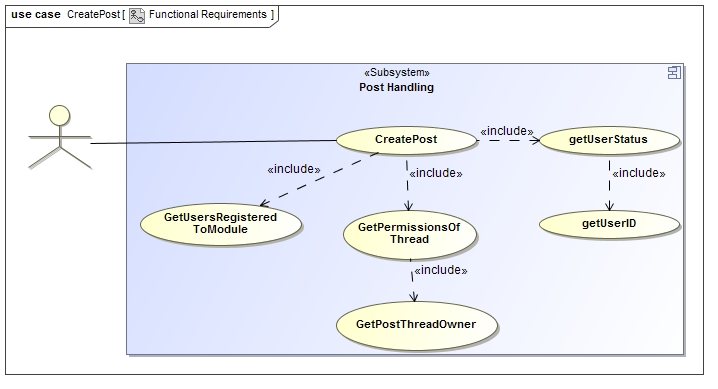
\includegraphics[width=1\linewidth]{./Images/PostHandling/postCreation.jpg}\\
\subsection{Process Specifications:} 

%MICHELLE
\section{Read Post}
\subsection*{Description:}This use case gives the functionality to read posts. A post will be marked as read/unread. Anyone can read any posts, if a user is not logged in, a guest account will be used to read posts.
\subsection{Prioritization:} Critical
\subsection{Conditions and Data Structures:}
\subsubsection*{Pre-Conditions:}None
\subsubsection*{Post-Conditions:}
\begin{itemize}
	\item If the user was logged in under his/her name, the post(s) that was/were read will be marked as unread.
	\item If a user was using the guest account, none of the posts will be marked/unmarked.
\end{itemize}
\subsubsection*{Requests and Results Data Structures:}
\subsection{Required Functionality:} 
\textbf{Use case diagram of the Read Post use case}\\
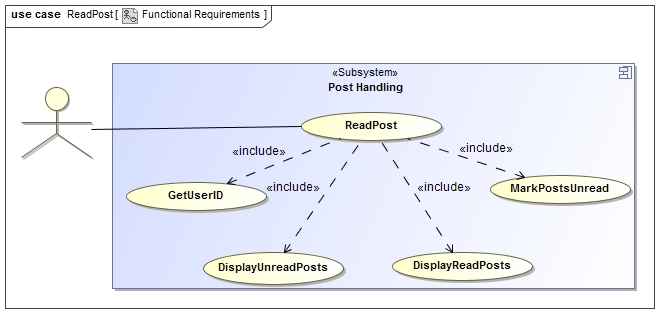
\includegraphics[width=1\linewidth]{./Images/PostHandling/postRead.jpg}\\
\subsection{Process Specifications:} 

%MICHELLE
\section{Update Post}
\subsection*{Description:}This use case refers to the ability to update posts that have already been posted. The user will have a specified time frame in which he/she will have the option to do this.  
\subsection{Prioritization:} Nice-to-have
\subsection{Conditions and Data Structures:}
\subsubsection*{Pre-Conditions:}
\begin{itemize}
	\item The user must be logged in.
	\item The user must be the original creator of the post.
\end{itemize}
\subsubsection*{Post-Conditions:}
\begin{itemize}
	\item The posts will be updated accordingly.
\end{itemize}
\subsubsection*{Requests and Results Data Structures:}
\subsection{Required Functionality:} 
\textbf{Use case diagram of the Update Post use case}\\
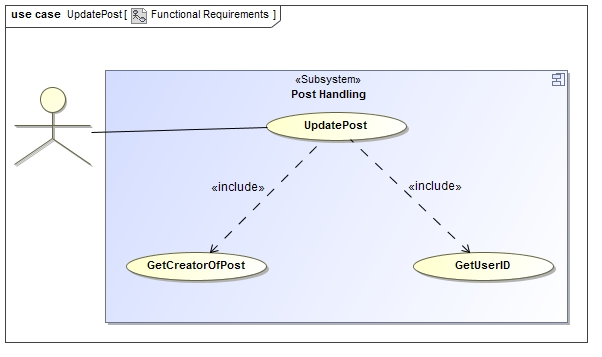
\includegraphics[width=1\linewidth]{./Images/PostHandling/postUpdate.jpg}\\
\subsection{Process Specifications:} 

%MICHELLE
\section{Delete Post}
\subsection*{Description:}This use case includes the ability to delete a post. Only the poster, creator of thread and other people with lecturer status will be able to do this.
This option will only be available if the user is logged in.
\subsection{Prioritization:}Important
\subsection{Conditions and Data Structures:}
\subsubsection*{Pre-Conditions:}
\begin{itemize}
	\item The user must be registered for the module.
	\item The user must be either the creator or a user with lecturer status.
\end{itemize}
\subsubsection*{Post-Conditions:}
\begin{itemize}
	\item The service will be rejected if the user is not registered for the specific module, or if the user is not the creator of the thread.
	\item If the deletion was successful, a message will be displayed to the user to notify him/her and the creator of the thread and/or the creator of thread will be informed of the deletion.
	\item Deleted post will be archived for future reference.
\end{itemize}
\subsubsection*{Requests and Results Data Structures:}
\subsection{Required Functionality:} 
\textbf{Use case diagram of the Delete Post use case}\\
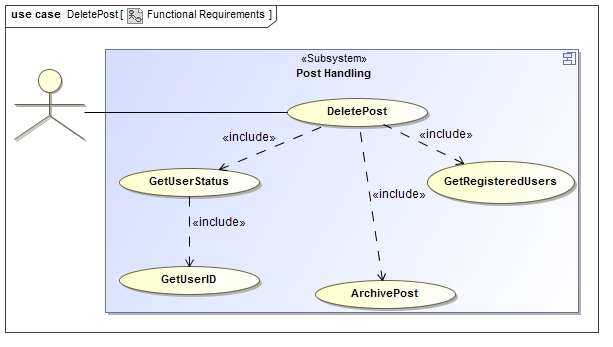
\includegraphics[width=1\linewidth]{./Images/PostHandling/postDeletion.jpg}\\
\subsection{Process Specifications:} 

%PRENOLAN
\section{Mark solution post}
\subsection*{Description:}
This use case allows a user or an owner of a thread to choose or mark a post in that thread as being the best answer, which should then elevate that post in the thread and should make in turn make the post easily visible as one enters the thread.
\subsection{Prioritization:} 
\textbf{Nice-To-Have}: Marking a post as the best answer.
\subsection{Conditions and Data Structures:}
\subsubsection*{Pre-Conditions:}
A user must have the privileges set by the administration of a space in order to mark a post as the best answer. The user is required to be logged in.
\subsubsection*{Post-Conditions:}
The thread should effectively display that an answer has been selected and optionally close the thread. The poster of the best answer should acquire an increase in progress to the next status level.
\subsubsection*{Requests and Results Data Structures:}
\includegraphics{Images/BestAnswer/Class_Diagram}
\subsection{Required Functionality:} 
\begin{center}
\includegraphics[width=0.9\linewidth]{./Images/BestAnswer/functional_requirements}
\end{center}
\subsection{Process Specifications:} 
\begin{center}
\includegraphics[width=1.2\linewidth]{./Images/BestAnswer/process_spec}
\end{center}

%PRENOLAN
\section{Vote and Evaluate Posts}
\subsection*{Description:}
This use case refers to the ability of a user to either vote up or down a post; a higher vote count on a post indicates the usefulness of a post. It also refers to a user being able to evaluate or give feedback on another users post.
\subsection{Prioritization:} 
\textbf{Important}: Voting on and evaluation of posts.
\subsection{Conditions and Data Structures:}
\subsubsection*{Pre-Conditions:}
A post has to have been created for a user to be able to vote on or evaluate it. Any user can vote on or evaluate a post as long as the user is logged in and a part of a specific Buzz Space. An exception to this rule is when the administration of a Buzz Space set specific rules as to which users (perhaps based on status) can vote on or evaluate posts.
\subsubsection*{Post-Conditions:}
A vote or evaluation has to be visible to every user (or only some based on the administration of that space) after it has been made on a post. A positive vote or evaluation has to reflect upon the posters progress to the next status level.
\subsubsection*{Requests and Results Data Structures:}
\includegraphics{Images/VotesAndEvaluation/Class_Diagram__Input}
\includegraphics{Images/VotesAndEvaluation/Class_Diagram__Output}
\subsection{Required Functionality:} 
\begin{center}
\includegraphics[width=0.9\linewidth]{./Images/VotesAndEvaluation/functional_requirements}
\end{center}
\subsection{Process Specifications:} 
\begin{center}
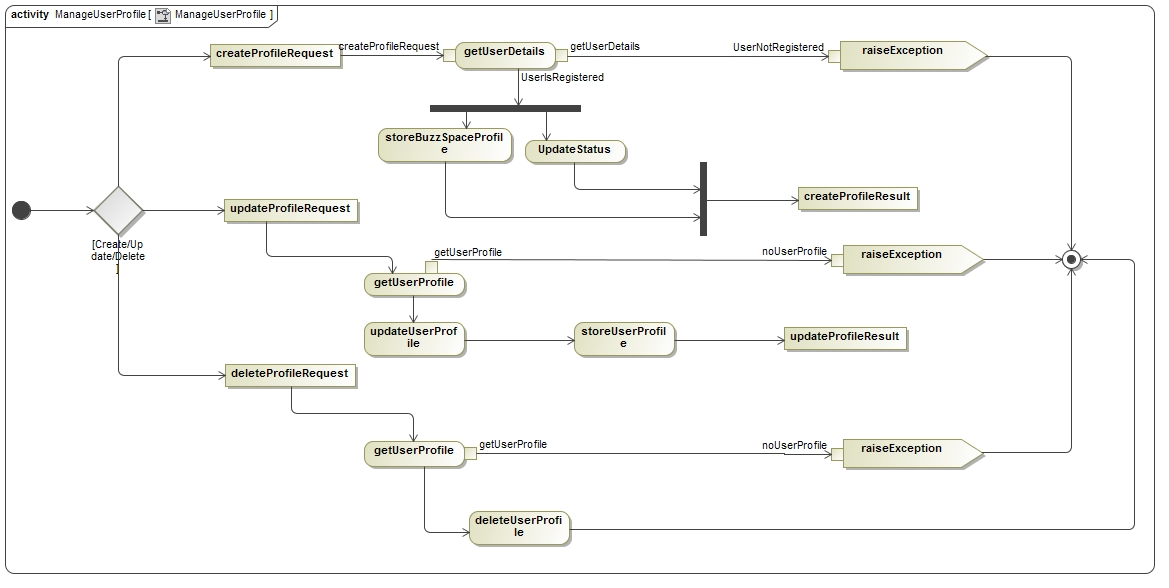
\includegraphics[width=1\linewidth]{./Images/VotesAndEvaluation/process_specification}
\end{center}

%MARIA
\section{Post Tagging}
\subsection*{Description:}
\textbf{Brief}:One very important functional requirement is the ability for the user to structure the information and content according to his own preference and needs. Social tagging is the feature that will enable him to do so
\subsection{Prioritization:} 
\textbf{Case-Priority - Important}: The user should be able to tag topics of interest in the post they created, as well
as posts created by other users.
\\Social tagging saves time and keeps user up to date with latest news and post regarding tagged topics
\\Users can: 
\\View posts according to tags.
\\Sort posts according to tags.
\\Follow different authors of posts and index topics and subjects according to tags.
\subsection{Conditions and Data Structures:}
\subsubsection*{Pre-Conditions:}
\textbf A post must not have been previously marked as a tag. If there are any keywords that look like "links" and have a hash symbol in front of them within the post, that post may be seen as already tagged.
\subsubsection*{Post-Conditions:}
\textbf A post becomes a tagged post if it has words with in it that have a hash symbol in front of them.
\\ words that are tags must change colour and become links.
\\The user can now index topics, follow different authors, sort and view posts according to the tagged topics.

\subsubsection*{Requests and Results Data Structures:}

\begin{center}
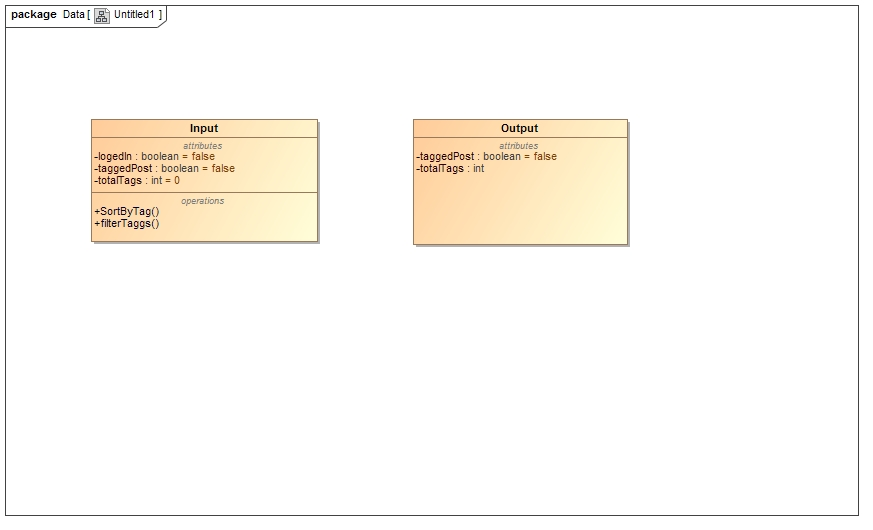
\includegraphics[width=0.9\linewidth]{Images/SocialTagging/Tag_Input_Output_ClassDiagram}
\end{center}

\textbf Figure 1: Input and Output classes showing potential attributes and operations *logedIn: boolean = true.

\subsection{Required Functionality:} 
\begin{center}
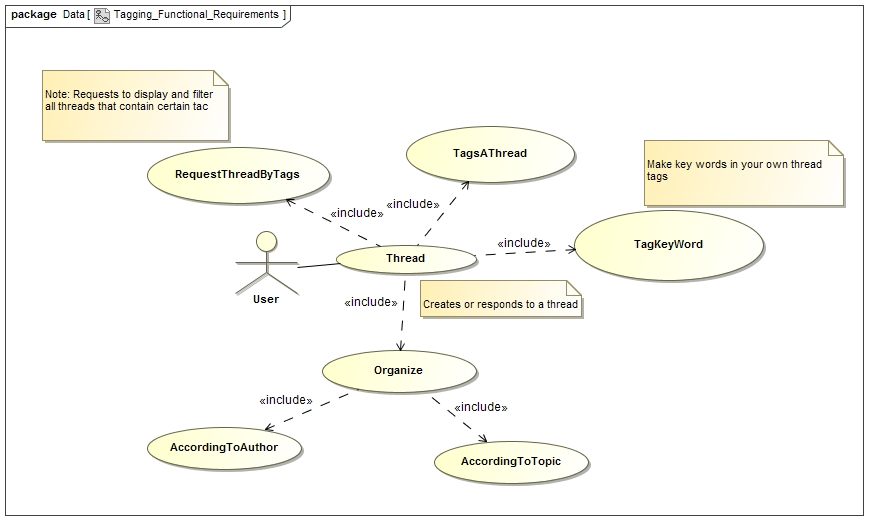
\includegraphics[width=0.9\linewidth]{Images/SocialTagging/Tagging_Functional_Requirements}
\end{center}

\textbf Figure 2: A UML use case diagram showing the required functionality for tagging posts.

\subsection{Process Specifications:} 

\begin{center}
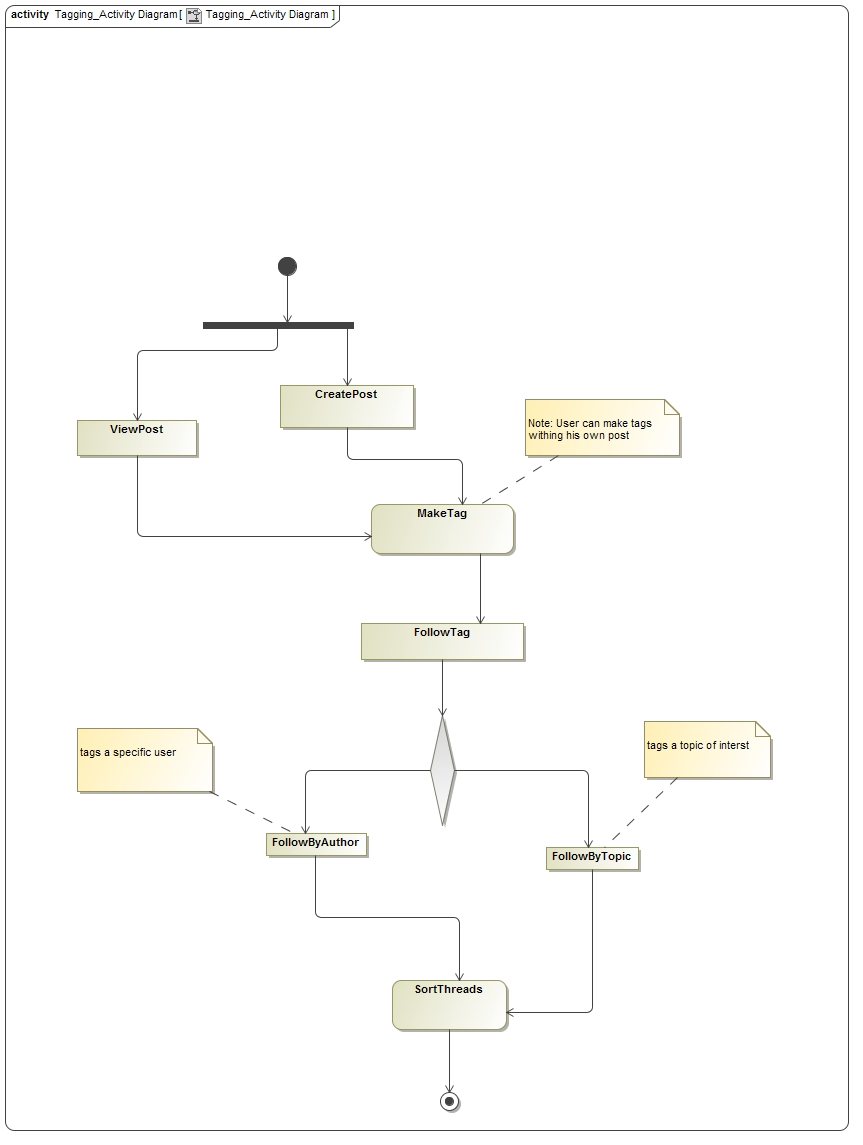
\includegraphics[width=0.9\linewidth]{Images/SocialTagging/Tagging_Activity_Diagram}
\end{center}

\textbf Figure 3: An activity diagram showing the process in which tags are made and organized. 

%LEAVE
\newpage
\begin{center}
\section*\textbf\huge{Filtering}
\addcontentsline{toc}{section}{Filtering}
\\
\Large{Use Cases}
\end{center}
\setcounter{section}{0}
%---------------------------------------------------------------START EDITING HERE FOR FILTERING----------------------------------------------------------------------
%THABANG
\section{Filter threads and buzzspaces}
\subsection*{Description:} This module provides a search and filter functionality.It allows the user to search the current Buzz Space they are in and if need be, filter the results. Users can filter the Buzz Space by tags, date,user or by user-rating. They can also search through the Buzz Space by entering a search-phrase in a search box, alternatively they can both search and filter i.e filter the search-results by tags, date, user or user-rating.\\
\subsection{Prioritization:} Since the number of threads can be infinitely high, this functionality is important when one wishes to view specific threads\\
\subsection{Conditions and Data Structures:}
\subsubsection*{Pre-Conditions:}
1.A specific Buzz Space has to have been created for a user to be able to search and/or filter.\\
2.The user has to atleast choose a single filter option and/or enter a search phrase\\
\subsubsection*{Post-Conditions:}
1.Upon clicking the submit button, the search and/or filter results will be automatically displayed for the user to see.\\
\subsubsection*{Requests and Results Data Structures:}
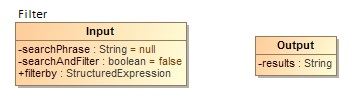
\includegraphics{Images/SearchAndFilter/Filter_input_output}\\
\includegraphics{Images/SearchAndFilter/Search_Input_output}\\
\includegraphics{Images/SearchAndFilter/SearchAndFilter_input_output}\\
\subsection{Required Functionality:} 
\includegraphics{Images/SearchAndFilter/SearchAndFilter_usecase}\\
\subsection{Process Specifications:} 
\includegraphics{Images/SearchAndFilter/Search_processSpecification}\\
\includegraphics{Images/SearchAndFilter/Filter_processSpecification}\\
\includegraphics{Images/SearchAndFilter/SearchAndFilter_processSpecification}\\

%LEAVE
\newpage
\begin{center}
\section*\textbf\huge{Authorisation}
\addcontentsline{toc}{section}{Authorisation}
\\
\Large{Use Cases}
\end{center}
\setcounter{section}{0}
%---------------------------------------------------------------START EDITING HERE FOR AUTHORISATION----------------------------------------------------------------------

\textbf{Overview}\\
\includegraphics[width=1\linewidth]{./Images/OverviewDiagrams/AuthorizationOverview.jpg}\\
%MICHELLE
\section{Login}
\subsection*{Description:}This use case defines the ability for a user to log into her/his account to activate certain functionalities of the system.
\subsection{Prioritization:}Critical
\subsection{Conditions and Data Structures:}
\subsubsection*{Pre-Conditions:}
\begin{itemize}
	\item The user must be a registered student.
\end{itemize}
\subsubsection*{Post-Conditions:}
\begin{itemize}
	\item If the user is not registered, an exception will be thrown and an error message will be shown to the user.
	\item If the login was successful, a message will be shown to inform the user that he/she is now logged in. More features will now be available to the user.
\end{itemize}
\subsubsection*{Requests and Results Data Structures:}
\subsection{Required Functionality:} 
\subsection{Process Specifications:} 

%JESSICA
\section{Logout}
\subsection*{Description:}
1.	User activates “Logout” function by selecting the “Logout” option.\\
2.	System responds by presenting user with standard Guest interface with no profile or privileges\\
\subsection{Prioritization:}
This Use case is considered Important\\ 
\subsection{Conditions and Data Structures:}
Participants:\\
Initiated by User and communicates with system\\
\subsubsection*{Pre-Conditions:}
1.	The user must click on “Logout” function\\
\subsubsection*{Post-Conditions:}
1.	System displays user with standard guest interface\\
2.	User has no privileges and status and cannot perform any function that a logged in user can\\
\subsubsection*{Requests and Results Data Structures:}
\includegraphics[width=1\linewidth]{./Images/CRUDThread/Diagrams/17.jpg}\\
Steps:\\
1.	User selects the logout option\\
1.1.	Boolean field in the specific user class – e.g User3 will be switched to false\\
2.	User will be presented with Guest interface\\
\subsection{Required Functionality:} 
\includegraphics[width=1\linewidth]{./Images/CRUDThread/Diagrams/18.jpg}\\
\subsection{Process Specifications:} 
Activity Diagram\\
\includegraphics[width=1\linewidth]{./Images/CRUDThread/Diagrams/19.jpg}\\
Sequence Diagram\\
\includegraphics[width=1\linewidth]{./Images/CRUDThread/Diagrams/20.jpg}\\

%MICHELLE
\section{Registration}
\subsection*{Description:}This use case gives the ability to register to a specific BuzzSpace.
\subsection{Prioritization:} Critical
\subsection{Conditions and Data Structures:}
\subsubsection*{Pre-Conditions:}
\begin{itemize}
	\item The user must be a registered student of the module associated with the BuzzSpace
\end{itemize}
\subsubsection*{Post-Conditions:}
\begin{itemize}
	\item If the user is not a registered student for the module, an exception is thrown and an error message is shown to the user.
	\item If the service was successful, a message is shown to the user to inform him/her that it was successful. The user will now be able to operate on the BuzzSpace.
\end{itemize}
\subsubsection*{Requests and Results Data Structures:}
\subsection{Required Functionality:} 
\subsection{Process Specifications:} 

%LEAVE
\newpage
\begin{center}
\section*\textbf\huge{Reporting}
\addcontentsline{toc}{section}{Reporting}
\\
\Large{Use Cases}
\end{center}
\setcounter{section}{0}
%---------------------------------------------------------------START EDITING HERE FOR REPORTING----------------------------------------------------------------------
%LUTFIYYA
%Thread Evaluation Report
\section{Thread Evaluation Report}
\subsection*{Description:}
This use case gives a user with certain privileges the ability to calculate statistical information about threads and to generate reports. The use case include the sourcing of all thread components, the calculating of statistics, construction of report data objects and the rendering of a report onto a user interface or PDF file.
\subsection{Prioritization:} 
\textbf{Important}: Thread Evaluation Report
\subsection{Conditions and Data Structures:}
\subsubsection*{Pre-Conditions:}
A user has to be a registered user of a Buzz Space and must also be logged in to be able to generate a report. The ThreadID has to exist.\\
\subsubsection*{Post-Conditions:}
A user should get statistical information about threads and generate a threads evaluation report.\\
\subsubsection*{Requests and Results Data Structures:}
\includegraphics{Images/Report/Input&Output}
\subsection{Required Functionality:} 
\includegraphics[width=15cm,height=10cm]{./Images/Report/Thread_FR}\\
\\
\subsection{Process Specifications:} 
\includegraphics[width=15cm,height=10cm]{./Images/Report/ThreadReport_PS}

%Student Post Report
\section{Student Post Evaluation Report}
\subsection*{Description:}
This use case gives a user with certain privileges the ability to calculate statistical information about students and posts. They can also generate reports. The use case include the sourcing of all student and post components, the calculating of statistics, construction of report data objects and the rendering of a report onto a user interface or PDF file. Users request sufficient information to identify the student and the post. The response object has a timestamp.
\subsection{Prioritization:} 
\textbf{Important}: Student and Post Evaluation Report
\subsection{Conditions and Data Structures:}
\subsubsection*{Pre-Conditions:}
A user has to be a registered user of a Buzz Space and must also be logged in to be able to generate a report. The UserID and post has to exist within a given Buzz Space.\\
\subsubsection*{Post-Conditions:}
A user should get statistical information about students and posts as well as a student post evaluation report.\\
\subsubsection*{Requests and Results Data Structures:}
\includegraphics{Images/Report/Input&Output}
\subsection{Required Functionality:} 
\includegraphics[width=15cm,height=10cm]{./Images/Report/studentPost_FR}\\
\\
\subsection{Process Specifications:} 
\includegraphics[width=15cm,height=10cm]{./Images/Report/StudentPost_PS}

%Audit Report
\section{Audit Report}
\subsection*{Description:}
This use case gives a lecturer the ability to generate an audit report for any thread, post or student, which will contain:
\begin{itemize}
\item A data/time stamp
\item User contributions
\item ThreadID for a specific thread
\item UserID for a specific user
\item Action which was performed by a user
\item All thread creations, modifications, deletions or updates
\item All user profile creations, modifications, deletions or updates
\item All post creations, modifications, deletions
\item All tag creations and usage
\item The number of votes per post
\item Users status levels and privileges
\item Any request to open/close a thread
\item Any request to generate any report including Thread Evaluation Report and Student Post Report
\end{itemize}

\subsection{Prioritization:} 
\textbf{Important}: Audit Report
\subsection{Conditions and Data Structures:}
\subsubsection*{Pre-Conditions:}
A lecturer has to be a registered user of a Buzz Space and must also be logged in to be able to generate a report.\\
\subsubsection*{Post-Conditions:}
A lecturer should get a detailed audit report.\\
%\subsubsection*{Requests and Results Data Structures:}
%\includegraphics{Images/Report/Input&Output}

%LEAVE
\newpage
\begin{center}
\section*\textbf\huge{Profile Handling}
\addcontentsline{toc}{section}{Proflie Handling}
\\
\Large{Use Cases}
\end{center}
\setcounter{section}{0}
%---------------------------------------------------------------START EDITING HERE FOR PROFILE HANDLING----------------------------------------------------------------------

%EPHI
\section{Create Profile}
\textbf{Overview}\\
\includegraphics[width=1\linewidth]{./Images/OverviewDiagrams/ProfileHandling.jpg}\\
\subsection*{Description:}
\textbf{Description:}Profile creation allows the user to register and login to the system to view and interact with the BuzzSpace.
\subsection{Prioritization:} 
\textbf{}Critical
\subsection{Conditions and Data Structures:}
\subsubsection*{Pre-Conditions:}
\begin{itemize}
\item User is logged into the system as a guest(There can only be on profile per user). 
\end{itemize}
\subsubsection*{Post-Conditions:}
\begin{itemize}
\item Validates a user logged into the system and has a new profile.
\end{itemize}
\subsubsection*{Requests and Results Data Structures:}
\includegraphics[width=1\linewidth]{./Images/UserProfile/CreateUserProfileStructure}
\subsection{Required Functionality:} 
\includegraphics[width=1\linewidth]{./Images/UserProfile/CreateUserProfileUseCase}
\subsection{Process Specifications:} 
\includegraphics[width=1\linewidth]{./Images/UserProfile/CreateUserProfileActivity}

%EPHI
\section{Modify Profile}
\subsection*{Description:}
\textbf{Description:}Profile modification allows the user logged into the system to modify the user profile that was previously created.
\subsection{Prioritization:}
\textbf{}Important
\subsection{Conditions and Data Structures:}
\subsubsection*{Pre-Conditions:}
\begin{itemize}
\item User logged into the system. 
\item User has an already existing profile. 
\end{itemize}
\subsubsection*{Post-Conditions:}
\begin{itemize}
\item User modifies existing profile: User is logged in and user profile has been modified. 
\item User keeps already existing profile: User had logged into the system and the profile had not been modified. 
\end{itemize}
\subsubsection*{Requests and Results Data Structures:}
\includegraphics[width=1\linewidth]{./Images/UserProfile/ModifyUserProfileStructure}
\subsection{Required Functionality:}
\includegraphics[width=1\linewidth]{./Images/UserProfile/ModifyUserProfileUseCase}
\subsection{Process Specifications:} 
\includegraphics[width=1\linewidth]{./Images/UserProfile/ModifyUserProfileActivity}


%EPHI
\section{View Profile}
\subsection*{Description:}
\textbf{Description:}Profile view allows the user to view ones or other users profiles on the BuzzSpace.
\subsection{Prioritization:} 
\textbf{}Nice To Have
\subsection{Conditions and Data Structures:}
\subsubsection*{Pre-Conditions:}
\begin{itemize}
\item User is logged into the system as a user not a guest. 
\end{itemize}
\subsubsection*{Post-Conditions:}
\begin{itemize}
\item The user is logged into the system and has a profile displayed.
\end{itemize}
\subsubsection*{Requests and Results Data Structures:}
\includegraphics[width=1\linewidth]{./Images/UserProfile/ViewUserProfileStructure}
\subsection{Required Functionality:} 
\includegraphics[width=1\linewidth]{./Images/UserProfile/ViewUserProfileUseCase}
\subsection{Process Specifications:} 
\includegraphics[width=1\linewidth]{./Images/UserProfile/ViewUserProfileActivity}

%EPHI
\section{Create Private Message}
\subsection*{Description:}
\textbf{Description}Create message allows the user that is logged into the system to create a messages such as email message, sms message and profile private message, and select the recipients then write of message contents and can include attachments to the message. 
\subsection{Prioritization:} 
\textbf{}Nice To Have
\subsection{Conditions and Data Structures:}
\subsubsection*{Pre-Conditions:}
\begin{itemize}
\item User is logged into the system as a user not a guest. 
\end{itemize}
\subsubsection*{Post-Conditions:}
\begin{itemize}
\item The user is logged into the system and has sent a message.
\end{itemize}
\subsubsection*{Requests and Results Data Structures:}
\subsection{Required Functionality:} 
\includegraphics[width=1\linewidth]{./Images/PrivateMessage/createMessageFunctionality}
\subsection{Process Specifications:} 
\includegraphics[width=1\linewidth]{./Images/PrivateMessage/createMessgeActivity}

%EPHI
\section{Read Private Message}
\subsection*{Description:}
\textbf{Description}Read message allows the user that is logged into the system to read a messages such as email message, sms message and profile private message that has been sent to them by a another BuzzSpace user.
\subsection{Prioritization:} 
\textbf{}Nice To Have
\subsection{Conditions and Data Structures:}
\subsubsection*{Pre-Conditions:}
\begin{itemize}
\item User is logged into the system as a user not a guest. 
\end{itemize}
\subsubsection*{Post-Conditions:}
\begin{itemize}
\item The user is logged into the system and has received one or more messages.
\end{itemize}
\subsubsection*{Requests and Results Data Structures:}
\subsection{Required Functionality:} 
\includegraphics[width=1\linewidth]{./Images/PrivateMessage/readMessageUseCase}
\subsection{Process Specifications:} 
%\includegraphics[width=1\linewidth]{./Images/PrivateMessage/createMessageActivity}

%EPHI
\section{Delete Private Message}
\subsection*{Description:}
\textbf{Description}Delete message allows the user that is logged into the system to delete a messages that has been sent to them by a another BuzzSpace user, a message that is out of date or is unimportant for the user, from their inbox.
\subsection{Prioritization:} 
\textbf{}Nice To Have
\subsection{Conditions and Data Structures:}
\subsubsection*{Pre-Conditions:}
\begin{itemize}
\item User is logged into the system as a user not a guest. 
\item There are messages in the inbox to delete.
\end{itemize}
\subsubsection*{Post-Conditions:}
\begin{itemize}
\item The user is logged into the system and has deleted one or more messages.
\item The messages deleted are no longer available in the system.
\end{itemize}
\subsubsection*{Requests and Results Data Structures:}
\includegraphics[width=1\linewidth]{./Images/PrivateMessage/deleteMessageUseCase}
\subsection{Process Specifications:} 
\includegraphics[width=1\linewidth]{./Images/PrivateMessage/deleteMessageActivity}

%LEAVE
\newpage
\begin{center}
\section*\textbf\huge{Domain Model}
\addcontentsline{toc}{section}{Domain Model}

\end{center}
\setcounter{section}{0}
%---------------------------------------------------------------START EDITING HERE FOR DOMAIN MODEL----------------------------------------------------------------------

\end{document}

